\documentclass[article, 12pt, oneside, a4paper, brazil]{abntex2}

\usepackage{lmodern}
\usepackage[T1]{fontenc}
\usepackage[utf8]{inputenc}
\usepackage{lastpage}
\usepackage{indentfirst}
\usepackage{color}
\usepackage{graphicx}
\usepackage{microtype}
\usepackage{tabularx}
\usepackage{booktabs}

\definecolor{blue}{RGB}{41,5,195}
\hypersetup{
     	%pagebackref=true,
		pdftitle={\@title}, 
		pdfauthor={\@author},
    	pdfsubject={\imprimirpreambulo},
	    pdfcreator={LaTeX with abnTeX2},
		pdfkeywords={abnt}{latex}{abntex}{abntex2}{trabalho acadêmico}, 
		colorlinks=true,       		% false: boxed links; true: colored links
    	linkcolor=blue,          	% color of internal links
    	citecolor=blue,        		% color of links to bibliography
    	filecolor=magenta,      		% color of file links
		urlcolor=blue,
		bookmarksdepth=4
}

\setlength{\parindent}{1.3cm}
\setlength{\parskip}{0.2cm}
\makeindex

\begin{document}
\selectlanguage{brazil}
\frenchspacing

\pdfbookmark[0]{\contentsname}{toc}
\tableofcontents*
\cleardoublepage

 \section*{\textbf{Documento de Requisitos:} Sistema de Pedidos Eletrônico para Restaurantes com Controle de Fluxos de Produção e Programa de Fidelidade}
 \section{Introdução}
 
 \subsection{Propósito}
 O propósito deste documento de especificação de requisitos é definir todos os requisitos do Sistema de Pedidos Eletrônico para Restaurantes com Controle de Fluxos de Produção e Programa de Fidelidade, sistema que tem como objetivo principal gerenciar pedidos, controlar o fluxo de produção e informar os itens sendo produzidos aos clientes, bem como oferecer bonificações aos clientes baseado no histórico de compras.
 
 \subsection{Escopo}
 O sistema recebe os pedidos através de um atendente e os envia para a unidade produção, onde entram para o fluxo de produção de três estágios, sendo eles aguardando, em produção e pronto, sendo que tais informações são compartilhadas com os clientes.
 
 \subsection{Organização da Especificação de Requisitos de Software}
 
 Este documento está dividido em três seções. Na primeira seção, é apresentada uma breve introdução sobre o conteúdo deste documento. Na segunda seção, uma descrição geral do sistema é apresentada e na última seção são descritos, de forma detalhada, todos os requisitos funcionais e não-funcionais do sistema.
 
 \section{Descrição Geral do Sistema}
 O objetivo do sistema é receber os pedidos dos clientes através de um dispositivo móvel portado pelo atendente, o pedido é então analisado e enviado a unidade de produção, caso haja a falta de algum ingrediente para o preparo, o sistema deverá informar que o mesmo não pode ser pode ser produzido. 
 
 Após a aceitação do pedido, este é recebido na unidade de produção através do controle de fluxo de produção e entra para o estágio aguardando, assim que sua produção for iniciada, sua situação deve ser alterada para em produção e após finalizado para pronto. Tais informações também estarão disponíveis aos clientes por meio de um dispositivo de exibição. Uma cópia do pedido é impressa e entregue ao cliente e será utilizada para encerrar o processo.
 
 O pedido é finalizado quando o cliente efetua o seu pagamento, a identificação é realizada pelo número do pedido contido na cópia entregue a ele ou pelo número da mesa que estava ocupando, o cliente é identificado pelo seu número do CPF (Cadastro de Pessoas Físicas) e o pedido é salvo no histórico de compras. O histórico de compras visa oferecer bonificações baseadas nas regras de negócio.
 
 \subsection{Funções do Produto}
 O sistema apresenta como principal objetivo gerenciar o ciclo de produção em um restaurante, desde a realização até o pagamento do pedido, realizando as seguintes funções:
 
 \begin{itemize}
  \item Inclusão, alteração, exclusão e consulta de ingredientes;
  \item Inclusão, alteração, exclusão e consulta de produtos;
  \item Inclusão, alteração e consulta de pedidos;
  \item Inclusão e consulta de clientes;
  \item Emissão do histórico de compras por cliente;
 \end{itemize}

 \subsection{Características do Usuário}
 O sistema é destinado a três grupos de usuários, sendo eles: atendentes, cozinheiros e caixa. Sendo necessário ter uma noção básica sobre computadores.
 
 \subsection{Suposições e Dependências}
 A configuração mínima requerida para a execução do sistema é composta por dispositivos móveis portadores de android, dois microcomputadores, sendo um com tela sensível ao toque e o outro hospedando o sistema, por fim, uma televisão para exibir o estado dos pedidos.
 
 \section{Requisitos Específicos} 
 \subsection{Requisitos Funcionais}
 
 \subsection*{\emph{Cadastro de Ingredientes}}
 \begin{description}
  \item[RF1.] O sistema deve permitir a inclusão, alteração e remoção de ingredientes no sistema. Os dados de ingredientes consistem de: nome, preço, fornecedor, contato do fornecedor e quantidade em estoque.
  \item[RF2.] O sistema deve permitir o cadastro de apenas um ingrediente por nome.
  \item[RF3.] O sistema deve permitir apenas ao administrador incluir, alterar ou remover ingredientes.
 \end{description}

 \subsection*{\emph{Cadastro de Produtos}}
 \begin{description}
  \item [RF4.] O sistema deve permitir a inclusão, alteração e remoção de produtos no sistema. Os dados de produtos consistem de: número de identificação único, nome, preço, ingredientes e categoria.
  \item [RF5.] O sistema deve permitir a alteração dos dados do produto, exceto o número de identificação único.
  \item [RF6.] O sistema deve emitir mensagens de erro caso um produto seja adicionado aos pedidos e algum ingrediente esteja indisponível no estoque.
 \end{description}
 
 \subsection*{\emph{Cadastro de Pedidos}}
 \begin{description}
  \item [RF7.] O sistema deve permitir a inclusão e alteração dos pedidos. Os dados de pedido consistem de: número do pedido, produtos, valor total, identificação do cliente, data do pedido e estado do pedido.
  \item [RF8.] O sistema deve permitir a alteração dos dados do pedido, exceto o número do pedido, a identificação do cliente e a data do pedido.
  \item [RF9.] O sistema deve permitir a alteração do campo estado do pedido para: realizado, aprovado, aguardando, em produção, pronto e finalizado.
 \end{description}
 
 \subsection*{\emph{Cadastro de Clientes}}
 \begin{description}
  \item [RF10.] O sistema deve permitir a inclusão de clientes. Os dados de clientes consistem de: CPF, nome do cliente e pontos acumulados.
  \item [RF11.] O sistema deve permitir o cadastro de apenas um cliente por CPF.
 \end{description}
 
 \subsection*{\emph{Informações do Programa de Fidelidade}}
 \begin{description}
  \item [RF12.] O sistema deve permitir que um pedido esteja vinculado a apenas um cliente.
  \item [RF13.] O sistema deve permitir que apenas pedidos com o estado de finalizados sejam vinculados aos pontos acumulados do cliente.
 \end{description}
 
 \subsection*{\emph{Relatórios}}
 \begin{description}
  \item [RF14.] O sistema deve gerar relatórios de todos os pedidos realizados por cliente, data ou produto.
  \item [RF15.] O sistema deve gerar relatórios da quantidade de ingredientes em estoque.
 \end{description}
 
 \subsection{Requisitos Não-Funcionais}
 \begin{description}
  \item [RN1.] O sistema é composto por três (3) subsistemas, sendo eles: sistema para atendimento, sistema para fluxo de produção e sistema para caixa.
  \item [RN2.] O sistema deve ser capaz de realizar cópias de segurança de todos os dados do sistema.
  \item [RN3.] O sistema deve ser facilmente portável para os ambientes Linux e Windows.
 \end{description}

\begin{figure}[h]
 \centering
 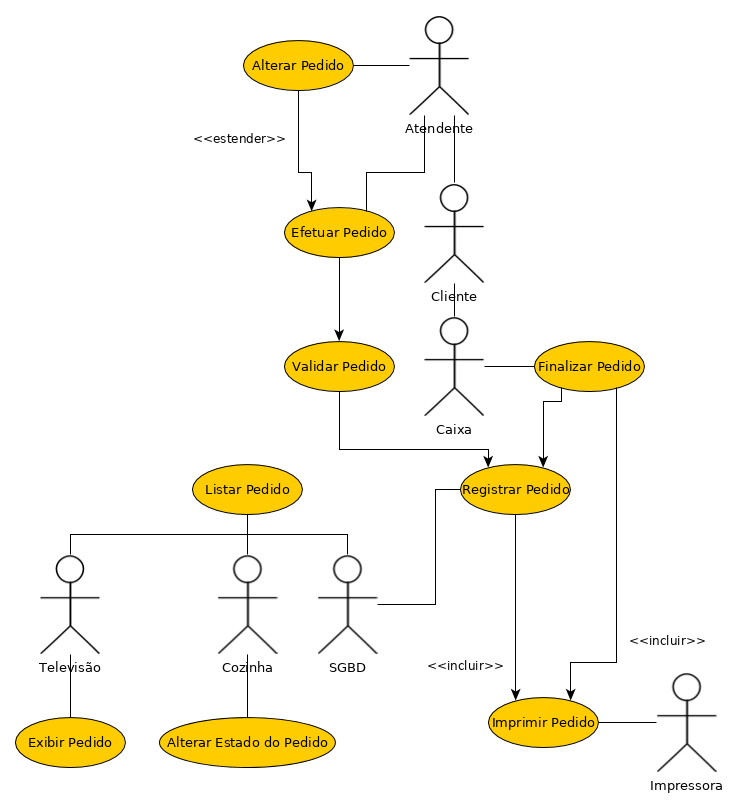
\includegraphics[scale=0.5]{images/imagem01.png}
\end{figure}

\begin{center}
 \begin{tabularx}{\textwidth}{lX}\specialrule{1.2pt}{1pt}{1pt}
  \textbf{Caso de Uso:} & Efetuar Pedido\\ \hline
  \textbf{Visão Geral:} & O cliente realiza o pedido dos itens desejados ao atendente, os itens são validados pelo sistema e o pedido é registrado. Após o registro, uma cópia do pedido é impressa e entregue ao cliente pelo atendente. O sistema envia o pedido à cozinha onde tem o seu estado atualizado de acordo com o fluxo de produção. Quando finalizado, o produto é entregue ao cliente pelo atendente e o sistema atualiza o estoque baseado nos itens do pedido.\\ \specialrule{1.2pt}{1pt}{1pt}
 \end{tabularx}
\end{center}

\begin{center}
 \begin{tabularx}{\textwidth}{lX}\specialrule{1.2pt}{1pt}{1pt}
  \textbf{Caso de Uso:} & Finalizar Pedido\\ \hline
  \textbf{Visão Geral:} & O cliente dirige-se ao caixa, apresenta sua via do pedido e informa seu CPF, o caixa informa os dados ao sistema, o sistema identica o cliente e o pedido e informa as bonificações disponíveis, o cliente efetua o pagamento e o sistema registra o pedido.  \\ \specialrule{1.3pt}{1pt}{1pt}
 \end{tabularx}
\end{center}

\begin{center}
 \begin{tabularx}{\textwidth}{lX}\specialrule{1.2pt}{1pt}{1pt}
  \textbf{Caso de Uso:} & Listar Pedido\\ \hline
  \textbf{Visão Geral:} & O sistema lista todos os pedidos com estado de aguardando, em produção e pronto. Os pedidos listados são exibidos e tem o estado alterado pela cozinha conforme forem sendo produzidos. A televisão informa aos clientes o estado dos pedidos.  \\ \specialrule{1.2pt}{1pt}{1pt}
 \end{tabularx}
\end{center}

\begin{center}
 \begin{tabularx}{\textwidth}{lX}\specialrule{1.2pt}{1pt}{1pt}
  \textbf{Descrição:} & Este caso de uso detalha como é realizada a inclusão de um pedido realizado pelo cliente no sistema.\\ \hline
  \textbf{Atores:} &  Cliente, Atendente, Impressora.\\ \hline
  \textbf{Inclusões:} & Imprimir Pedido.\\ \hline
  \textbf{Extensões:} & Alterar Pedido.\\ \hline
  \textbf{Pré-condições:} & Nenhuma. \\ \hline
  \textbf{Detalhes:} & \begin{enumerate}[wide, labelwidth=!, noitemsep]
                           \item O cliente escolhe os itens do seu pedido.
                           \item O atendente registra o pedido de um cliente.
                           \item O sistema registra o pedido no SGDB.
                           \item A impressora imprime a via do cliente do pedido.
                           \item O atendente entrega a impressão ao cliente.
                          \end{enumerate}
\\ \hline
  \textbf{Pós-condições:} & O pedido estará registrado no sistema e com estado de aguardando\\ \hline
  \textbf{Exceções:} & \\ \hline
  \textbf{Restrições:} & \\ \hline
  \textbf{Variantes:} & \\ \hline
  \textbf{Comentários:} &  \\ \specialrule{1.3pt}{1pt}{1pt}
 \end{tabularx}
\end{center}


\end{document}
